
\documentclass[aspectratio=169]{beamer}
\usetheme{Boadilla}

\usepackage{qrcode}

\usepackage[utf8]{inputenc}       % Codificação de entrada
\usepackage[T1]{fontenc}          % Codificação de saída
\usepackage[portuguese]{babel}   % Idioma
\usepackage{XCharter}             % Fonte principal
\AtBeginDocument{\fontsize{12}{12}\selectfont}

%\usepackage{geometry}
%\geometry{papersize={210mm,150mm}}
\usepackage{tikz}
\usepackage{pgf-pie} % necessário para gráficos de pizza

\usepackage{color}
\usepackage{graphicx}
\usepackage{amsmath, amssymb, amsfonts}
\usepackage{bm}
\usepackage{booktabs}
\usepackage{multirow}
\usepackage{caption}
\usepackage{subfigure}
\usepackage{wrapfig}
\usepackage{multicol}
\usepackage{sidecap}
\usepackage{tikz}
\usepackage{listings}
\usepackage{siunitx}
\usepackage{pdfpages}
\usepackage{float}
\usepackage{hyperref}
\usepackage{academicons}
\usepackage{setspace}

\newcommand{\eng}[1]{\textsl{#1}}
\newcommand{\cod}[1]{\texttt{#1}}

\usepackage{tikz}
\usetikzlibrary{shapes.geometric, arrows, positioning}

% Definição de estilos para o fluxograma
\tikzstyle{startstop} = [ellipse, rounded corners, minimum width=2cm, minimum height=0.8cm, text centered, draw=black, fill=gray!20]
\tikzstyle{process} = [rectangle, minimum width=3.5cm, minimum height=1cm, text width=4.5cm, text centered, draw=black, fill=white]
\tikzstyle{decision} = [diamond, aspect=2, minimum width=3cm, minimum height=1cm, text centered, draw=black, fill=white]
\tikzstyle{arrow} = [thick,->,>=stealth]

% Definição de cores profissionais
\definecolor{mipsblue}{RGB}{50, 90, 120}
\definecolor{mipsred}{RGB}{150, 30, 30}

\title[Arquitetura de Computadores]{\huge  Experimento 4} %note that the optional arg in '[]' are displayed in the left column throughout the complete presentation
% adapt accordingly
% e.g., M.Sc. Intermediate Thesis Report
% or     B.Sc. Intermediate Thesis Report


\author[Prof. Dr. Oscar Eduardo Anacona Mosquera]{Prof. Dr. Oscar Eduardo Anacona Mosquera \newline\newline 
	\scriptsize{oscar.mosquera@ufmt.br}
}%note that the optional arg in '[]' are displayed in the left column throughout the complete presentation



\AtBeginSection[]
{
	\begin{frame}{Sumário}
		\tableofcontents[currentsection]
	\end{frame}
}


\begin{document}

	\begin{frame}[plain]
		\titlepage
	\end{frame}
	
	\begin{frame}{Sumário}
		\tableofcontents
	\end{frame}
	
%=======================================================================================
%\section{Introdução}
%=======================================================================================


%\section{Introdução}




%\section{Contador Binário de 4 bits}

% --- SLIDE: CONCEITO ---
\begin{frame}{Contador de 4 bits}
    \justifying
    Um contador é um circuito sequencial que percorre uma sequência de estados a cada pulso de clock.
    
    \begin{itemize}
        \item \textbf{Capacidade}: 4 bits podem representar valores de 0 a 15 ($2^4 - 1$).
        \item \textbf{Componentes}: Registradores para armazenar o valor atual e um somador para calcular o próximo valor.
        \item \textbf{Overflow}: Ao chegar em 15, o próximo pulso de clock faz o contador voltar para 0 automaticamente.
    \end{itemize}
    
    \begin{block}{Biblioteca Arithmetic}
        Para somar em VHDL, utilizaremos a biblioteca \texttt{ieee.numeric\_std.all}.
    \end{block}
\end{frame}

% --- SLIDE: CODIGO VHDL CONTADOR ---
\begin{frame}[fragile]{Código VHDL: Contador de 32 bits}
\begin{lstlisting}[language=VHDL, basicstyle=\tiny]
library ieee;
use ieee.std_logic_1164.all;
use ieee.numeric_std.all; -- Necessaria para operacoes de soma

entity contador_4bits is
    port (
        clk    : in  std_logic;
        rst    : in  std_logic;
        q_out  : out std_logic_vector(31 downto 0)
    );
end entity;

architecture rtl of contador_4bits is
    signal count_reg : unsigned(31 downto 0) := (others => '0');
begin
    process(clk, rst)
    begin
        if rst = '0' then
            count_reg <= (others => '0');
        elsif rising_edge(clk) then
            count_reg <= count_reg + 1;
        end if;
    end process;

    q_out <= std_logic_vector(count_reg);
end architecture;
\end{lstlisting}
\end{frame}








% --- SLIDE: DESAFIO PRATICO ---
\begin{frame}{Desafio: Ligando na DE0-Nano}
    \justifying
    Para levar este projeto para a placa real, precisamos de um ajuste:
    
    \begin{alertblock}{Problema de Velocidade}
        O clock da DE0-Nano é de \textbf{50 MHz}. Se ligarmos os 8 bits do contador nos LEDs, eles piscarão tão rápido (milhões de vezes por segundo) que parecerão sempre acesos.
    \end{alertblock}

    \textbf{Como resolver?}
    \begin{itemize}
        \item Criar um contador de 32 bits.
        \item Ligar os LEDs nos bits mais significativos (ex: \texttt{count\_reg(25 downto 22)}).
        \item Isso fará com que os LEDs pisquem em uma frequência visível ao olho humano.
    \end{itemize}
\end{frame}






\begin{frame}{Solução Prática: Fluxo no Quartus }
	Para implementar essa divisão de clock via hardware, seguiremos o fluxo:
	
	\begin{enumerate}
		\item \textbf{Criação do Módulo:} Desenvolver o contador de 32 bits e usar a função \textit{Create Symbol Files for Current File}.
		\item \textbf{Design Esquemático (BDF):} 
		\begin{itemize}
			\item Instanciar o componente criado no arquivo \texttt{.bdf}.
			\item Duplicar ou conectar conforme a necessidade do projeto.
		\end{itemize}
		\item \textbf{Integração VHDL:} Converter o design para VHDL ou instanciar o arquivo de blocos em um \textit{wrapper} para simulação.
		\item \textbf{Configuração de Projeto:}
		\begin{itemize}
			\item Definir o arquivo principal (\textit{Set as Top-Level Entity}).
			\item Associar o \textit{Testbench} para validação funcional.
		\end{itemize}
	\end{enumerate}
\end{frame}



%\begin{frame}{Do Bloco à Simulação}
%	\begin{block}{1. Abordagem de Blocos (BDF)}
%		Ao criar um \textbf{Symbol}, podemos visualizar o contador como uma "caixa preta". No \texttt{.bdf}, conectamos o clock de 50MHz na entrada e derivamos os sinais:
%		\begin{itemize}
%			\item \texttt{count(25..22)} $\rightarrow$ Conectados aos LEDs físicos.
%		\end{itemize}
%	\end{block}
%	
%	\begin{block}{2. Verificação e Testbench}
%		Após instanciar os componentes:
%		\begin{itemize}
%			\item Geramos o arquivo VHDL equivalente para garantir a portabilidade.
%			\item \textbf{Top-Level:} Definimos qual módulo o Quartus deve compilar.
%			\item \textbf{Testbench:} Criamos o estímulo de clock para verificar se os bits mais significativos estão alternando no tempo esperado.
%		\end{itemize}
%	\end{block}
%\end{frame}
%






% --- PASSO 1: SYMBOLS (PARTE A) ---
\begin{frame}{Passo 1: Criação de Componentes (Symbols)}
	Para usar o design visual (BDF), primeiro transformamos o código VHDL em um bloco gráfico:
	\begin{itemize}
		\item Abra o arquivo de código fonte \texttt{.vhd}.
		\item Vá ao menu: \textbf{File $\rightarrow$ Create/Update}.
		\item Selecione: \textbf{Create Symbol Files for Current File}.
	\end{itemize}
	\begin{center}
		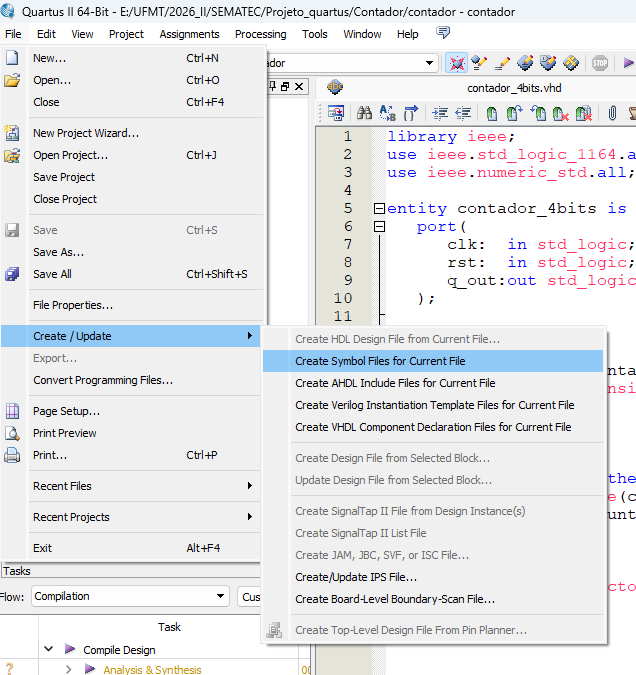
\includegraphics[width=0.3\textwidth]{Figs/fig01.png}
	\end{center}
\end{frame}

% --- PASSO 1: SYMBOLS (PARTE B) ---
\begin{frame}{Passo 1: Resultado do Symbol}
	\begin{itemize}
		\item O Quartus gera um arquivo \texttt{.bsf}.
		\item Esse "bloco" agora possui as entradas (\textit{inputs}) e saídas (\textit{outputs}) definidas no VHDL.
	\end{itemize}
	\begin{center}
		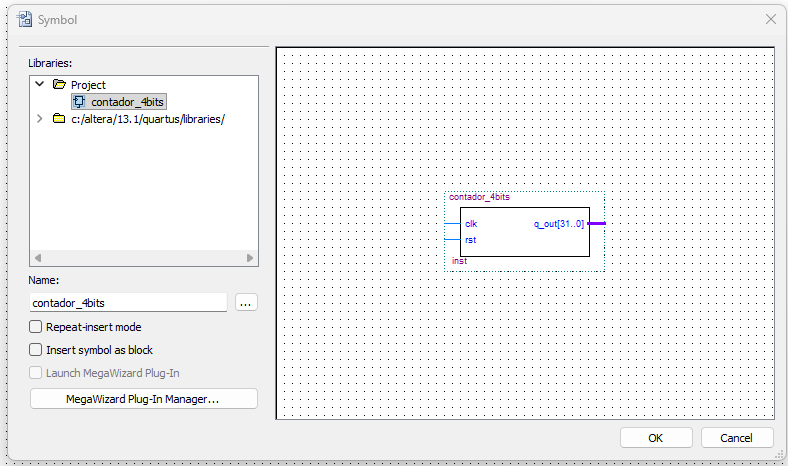
\includegraphics[width=0.7\textwidth]{Figs/fig04.png}
	\end{center}
\end{frame}

% --- PASSO 2: BDF (PARTE A) ---
\begin{frame}{Passo 2: Design Esquemático (BDF)}
	Criamos o arquivo de diagrama de blocos que será o top-level do projeto:
	\begin{itemize}
		\item Vá em \textbf{File $\rightarrow$ New}.
		\item Escolha \textbf{Block Diagram/Schematic File}.
	\end{itemize}
	\begin{center}
		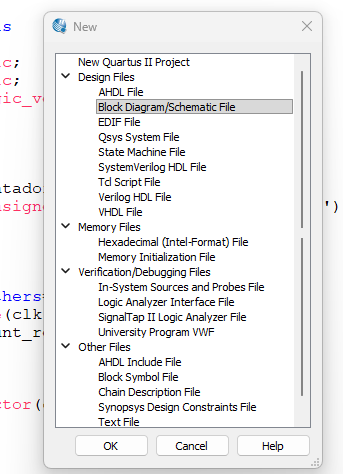
\includegraphics[width=0.3\textwidth]{Figs/fig02.png}
	\end{center}
\end{frame}

% --- PASSO 2: BDF (PARTE B) ---
\begin{frame}{Passo 2: Organização de Arquivos}
	No \textbf{Project Navigator}, você verá o arquivo \texttt{.bdf} integrado ao projeto junto com os arquivos VHDL:
	\begin{center}
		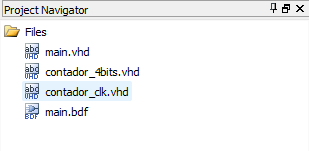
\includegraphics[width=0.6\textwidth]{Figs/fig10.png}
	\end{center}
\end{frame}

% --- PASSO 3: CONEXÕES (PARTE A) ---
\begin{frame}{Passo 3: Instanciação e Facilidades}
	Para não precisar criar pino por pino manualmente:
	\begin{itemize}
		\item Clique com o botão direito sobre o bloco inserido.
		\item Selecione \textbf{Generate Pins for Symbol Ports}.
	\end{itemize}
	\begin{center}
		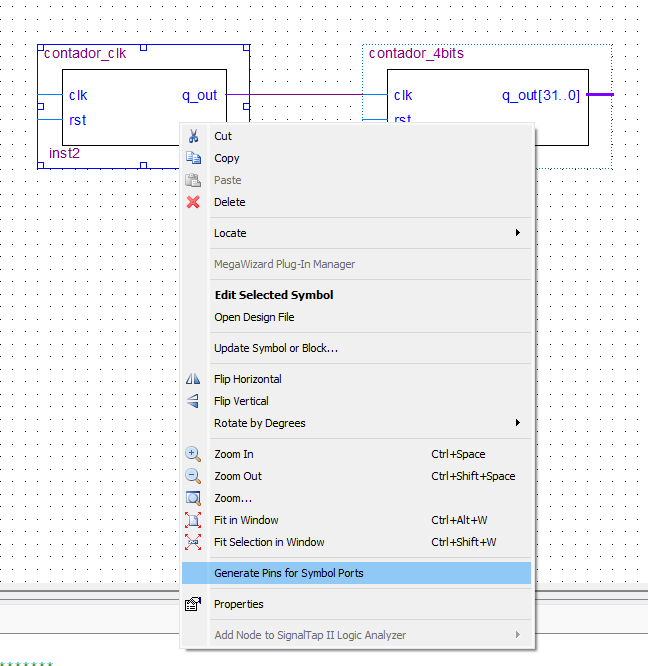
\includegraphics[width=0.4\textwidth]{Figs/fig06.png}
	\end{center}
\end{frame}

% --- PASSO 3: CONEXÕES (PARTE B) ---
\begin{frame}{Passo 3: Esquema Final Conectado}
	Interligamos os blocos (Ex: \texttt{contador\_clk} em série com \texttt{contador\_4bits}) para formar a lógica final de divisão de frequência:
	\begin{center}
		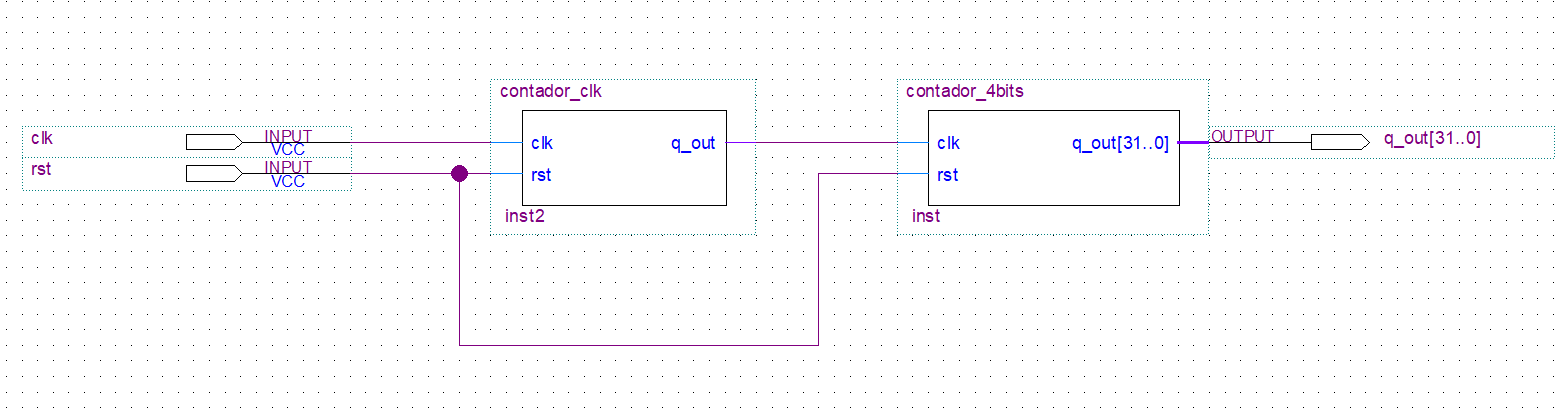
\includegraphics[width=\textwidth]{Figs/fig07.png}
	\end{center}
\end{frame}

% --- PASSO 4: PIN PLANNER (PARTE A) ---
\begin{frame}{Passo 4: Pin Planner (Visão da FPGA)}
	Após realizar a \textit{Analysis \& Elaboration}, acessamos o Pin Planner para visualizar o encapsulamento físico do Cyclone IV:
	\begin{center}
		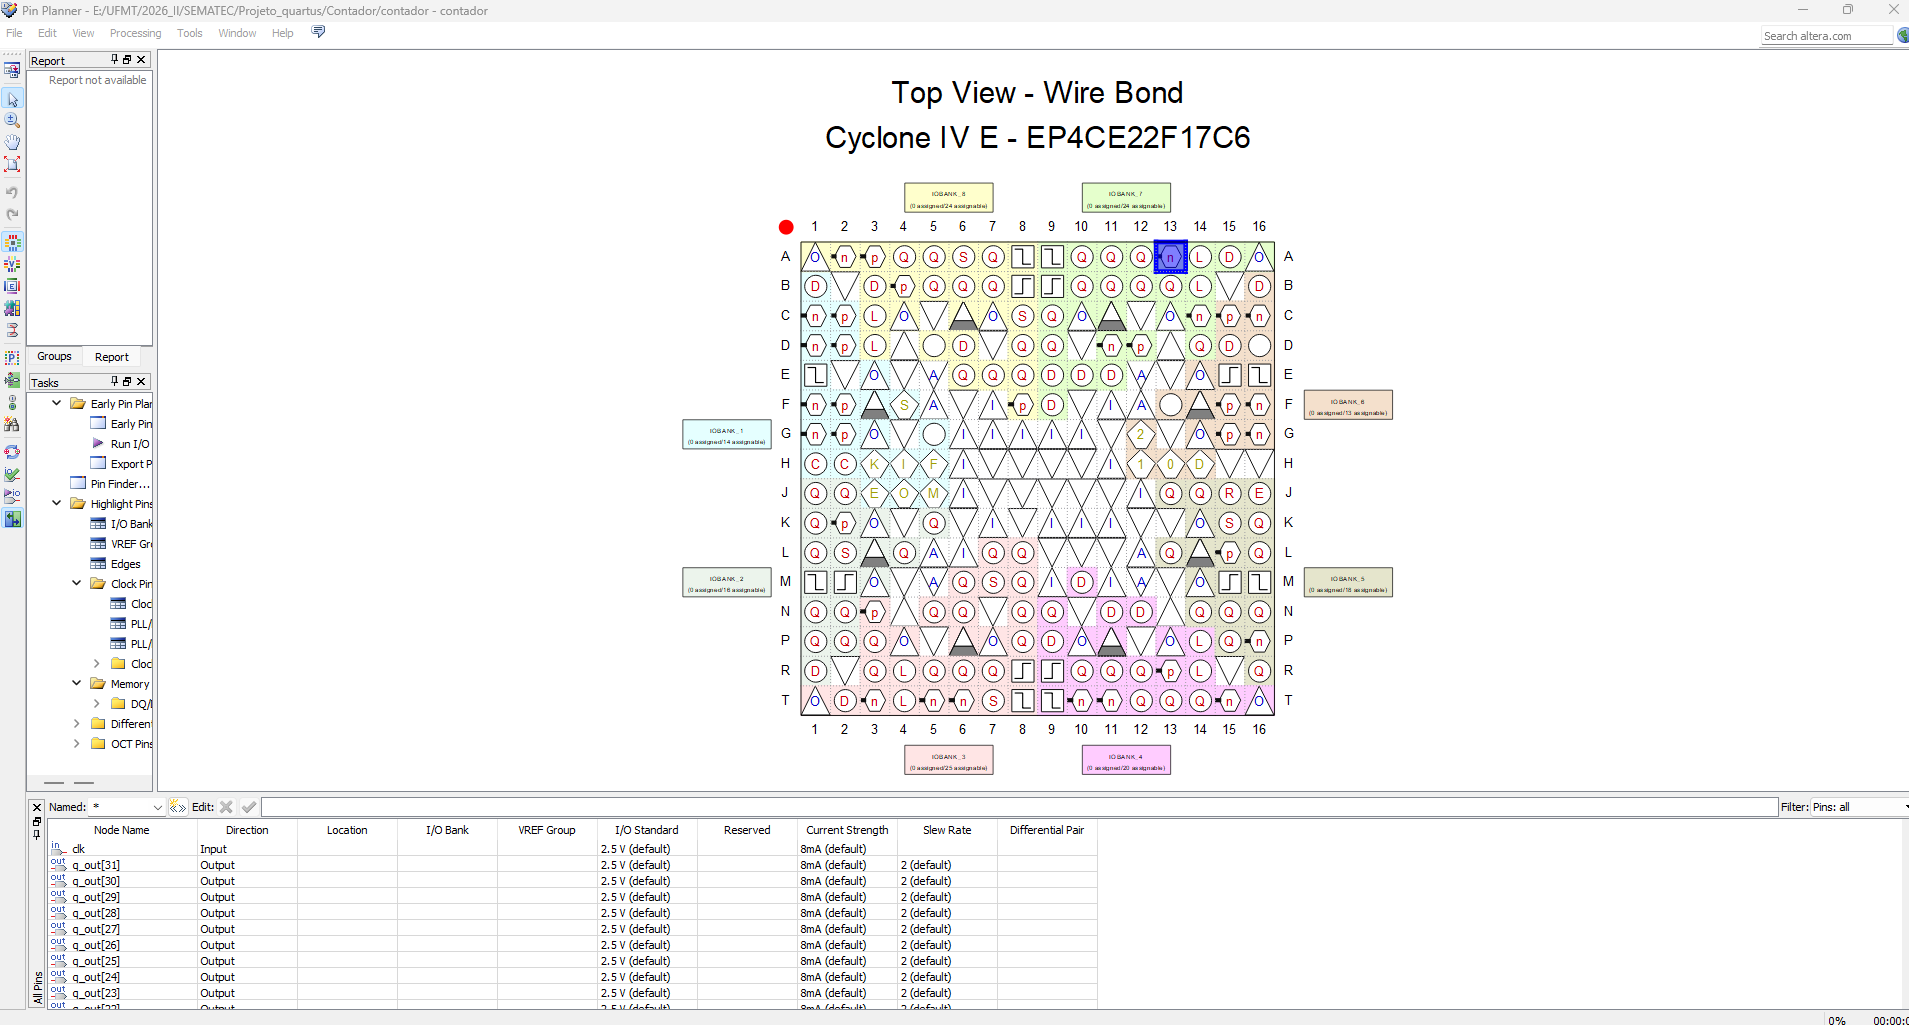
\includegraphics[width=1.2\textheight]{Figs/fig12.png}
	\end{center}
\end{frame}

% --- PASSO 4: PIN PLANNER (PARTE B) ---
\begin{frame}{Passo 4: Mapeamento de Pinos}
	Associamos os nomes lógicos aos pinos físicos da DE0-Nano (PIN\_R8, PIN\_J15, etc.):
	\begin{center}
		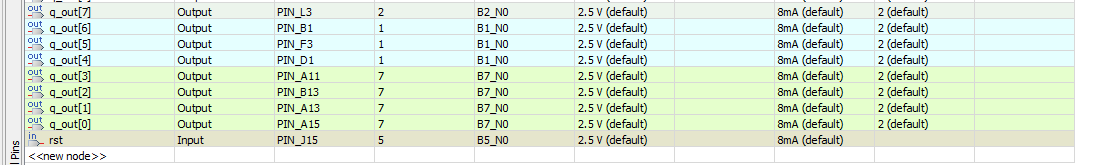
\includegraphics[width=\textwidth]{Figs/fig14.png}
	\end{center}
\end{frame}


\begin{frame}{Passo 4: Mapeamento de Pinos}
	Associamos os nomes lógicos aos pinos físicos da DE0-Nano (PIN\_R8, PIN\_J15, etc.):
	\begin{center}
		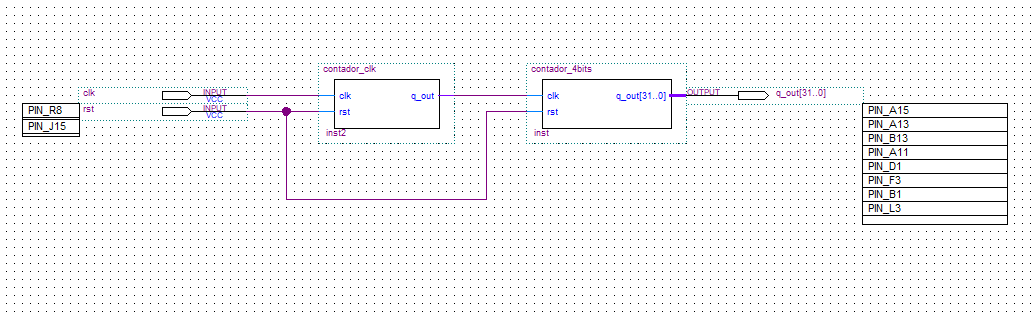
\includegraphics[width=\textwidth]{Figs/fig15.png}
	\end{center}
\end{frame}



% --- PASSO 5: FINALIZAÇÃO (PARTE B) ---
\begin{frame}{Passo 5: Exportação para HDL}
Podemos converter o BDF de volta para VHDL:
	\begin{itemize}
		\item \textbf{File $\rightarrow$ Create/Update}.
		\item \textbf{Create HDL Design File from Current File}.
	\end{itemize}
	\begin{center}
		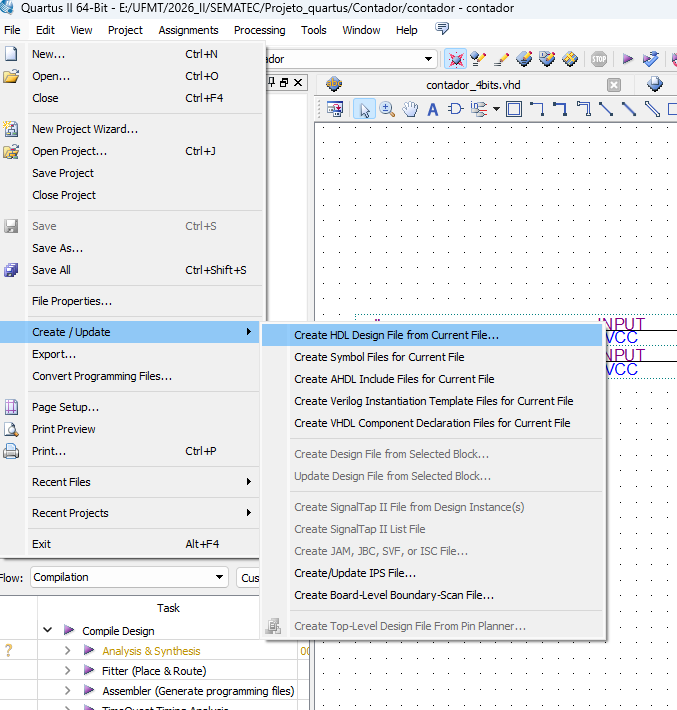
\includegraphics[width=0.35\textwidth]{Figs/fig08.png}
	\end{center}
\end{frame}









% --- PASSO 5: FINALIZAÇÃO (PARTE A) ---
\begin{frame}{Passo 5: Definindo a Entidade Top-Level}
	O Quartus precisa saber qual arquivo é a "raiz" do projeto para a compilação:
	\begin{itemize}
		\item Clique com o botão direito no arquivo principal.
		\item Selecione \textbf{Set as Top-Level Entity}.
	\end{itemize}
	\begin{center}
		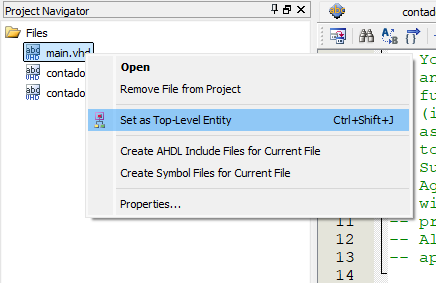
\includegraphics[width=0.5\textwidth]{Figs/fig11.png}
	\end{center}
\end{frame}






% --- SLIDE: TESTBENCH CONTADOR ---
\begin{frame}[fragile]{Testbench do Contador}
	\justifying
	O testbench apenas precisa gerar o clock e dar um pulso inicial no reset. O contador fará o resto do trabalho.
	
	\begin{lstlisting}[language=VHDL, basicstyle=\tiny]
		-- No processo de estimulo
		stim_proc: process
		begin
		rst <= '0'; 
		wait for 45 ns; -- Pulso de reset inicial
		rst <= '1';
		
		-- Deixamos o clock rodar por um longo tempo
		wait for 500 ns;
		
		wait;
		end process;
	\end{lstlisting}
	
	\begin{itemize}
		\item \textbf{Observação}: O sinal de clock é o mesmo processo do exemplo anterior (período de 20ns).
	\end{itemize}
\end{frame}



% --- SLIDE: ANALISE NO MODELSIM ---
\begin{frame}{Análise no ModelSim: Radix e Ondas}
	\justifying
	Para validar o contador, utilizaremos as ferramentas de visualização do ModelSim:
	
	\begin{enumerate}
		\item \textbf{Mudança de Radix}: Clique com o botão direito no sinal \texttt{q\_out} $\rightarrow$ \textit{Radix} $\rightarrow$ \textit{Unsigned}. Isso mostrará os números "0, 1, 2, 3..." em vez de bits.
		\item \textbf{Visualização Analógica}: Clique com o botão direito $\rightarrow$ \textit{Format} $\rightarrow$ \textit{Analog (automatic)}. Você verá uma escada (ramp) subindo conforme o contador incrementa.
		%\item \textbf{Reset}: Observe como o contador para imediatamente e volta ao zero quando o sinal \texttt{rst} vai para '1'.
	\end{enumerate}
	
	%\begin{figure}
	%\includegraphics[width=0.7\textwidth]{modelsim_contador_wave.png}
	%\caption{Contador incrementando a cada borda de subida.}
	%\end{figure}
\end{frame}



\begin{frame}{ModelSim}
	\justifying
	Para validar o contador, utilizaremos as ferramentas de visualização do ModelSim:
	
%	\begin{enumerate}
%		\item \textbf{Mudança de Radix}: Clique com o botão direito no sinal \texttt{q\_out} $\rightarrow$ \textit{Radix} $\rightarrow$ \textit{Unsigned}. Isso mostrará os números "0, 1, 2, 3..." em vez de bits.
%		\item \textbf{Visualização Analógica}: Clique com o botão direito $\rightarrow$ \textit{Format} $\rightarrow$ \textit{Analog (automatic)}. Você verá uma escada (ramp) subindo conforme o contador incrementa.
%		%\item \textbf{Reset}: Observe como o contador para imediatamente e volta ao zero quando o sinal \texttt{rst} vai para '1'.
%	\end{enumerate}
	
	\begin{figure}
	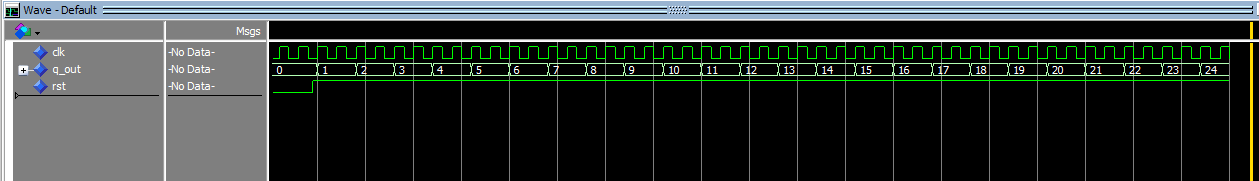
\includegraphics[width=0.9\textwidth]{Figs/fig16.png}
	%\caption{Contador incrementando a cada borda de subida.}
	\end{figure}
\end{frame}








% --- SLIDE: PARALELISMO REAL ---
\begin{frame}{O Diferencial: Paralelismo Real}
	\begin{block}{Hardware vs. Software}
		Diferente de um microcontrolador que simula paralelismo alternando tarefas rapidamente (sequencial), no FPGA o paralelismo é \textbf{físico}.
	\end{block}
	
	\textbf{Por que instanciar vários contadores?}
	\begin{itemize}
		\item Cada contador criado no BDF é um circuito independente e físico dentro do silício.
		\item Se tivermos 1 ou 100 contadores, todos incrementarão no \textbf{exato mesmo pulso de clock}.
		\item \textbf{Sem latência adicional:} Adicionar mais contadores não "deixa o sistema mais lento" (diferente de um código C onde mais loops consomem mais tempo de CPU).
	\end{itemize}
	
	\begin{alertblock}{Potencial de Observação}
		Ao ligar contadores em paralelo com diferentes seleções de bits para os LEDs, podemos observar diferentes frequências ocorrendo simultaneamente, de forma totalmente independente .
	\end{alertblock}
\end{frame}






\end{document}
